\subsection*{Gaussian Process with Rational Quadratic Kernel}

As a final study for the HEG, let us use the Gaussian process (GP) algorithm, another Bayesian machine learning algorithm, as the machine learning component in an SRE analysis. Here we will be using Gaussian processes as the machine learning component of the SRE algorithm. The kernel function will be a modified rational quadratic kernel consisting of a constant kernel multiplied by a rational quadratic kernel and then added to a white kernel. All kernels and the GP algorithm are implemented using the Python library Scikit-Learn.  

As a first study, we will use the same training data set as before, 16 training points taken from between 5 and 20 open shells. We will use an SRE sequence length of three for this training. The only other parameter we set is the $\alpha$ value of the GP algorithm, which we set to $\delta y_{train}^4$, where $\delta y_{train}$ is the standard deviation y component of the training data set. Using the standard deviation when setting $\alpha$ seems to keep the resulting uncertainties small but has little effect on the prediction results.

Fig. \ref{fig:gp_16_points} shows the analysis results on the same data set used in the Bayesian ridge regression section. The average percent error between the SRE predictions for the converged correlation energies and the fully calculated correlation energies at M = 6,142 is 0.73$\%$. While this is larger than the error resulting from the Bayesian ridge regression analysis, it is still tiny and acceptable. Furthermore, it is essential to note that the uncertainties on this, represented by the shaded regions, are significantly smaller than those on the Bayesian ridge regression plot. This is because they are so small in places hidden entirely by the lines!

\begin{figure}
    \centering
    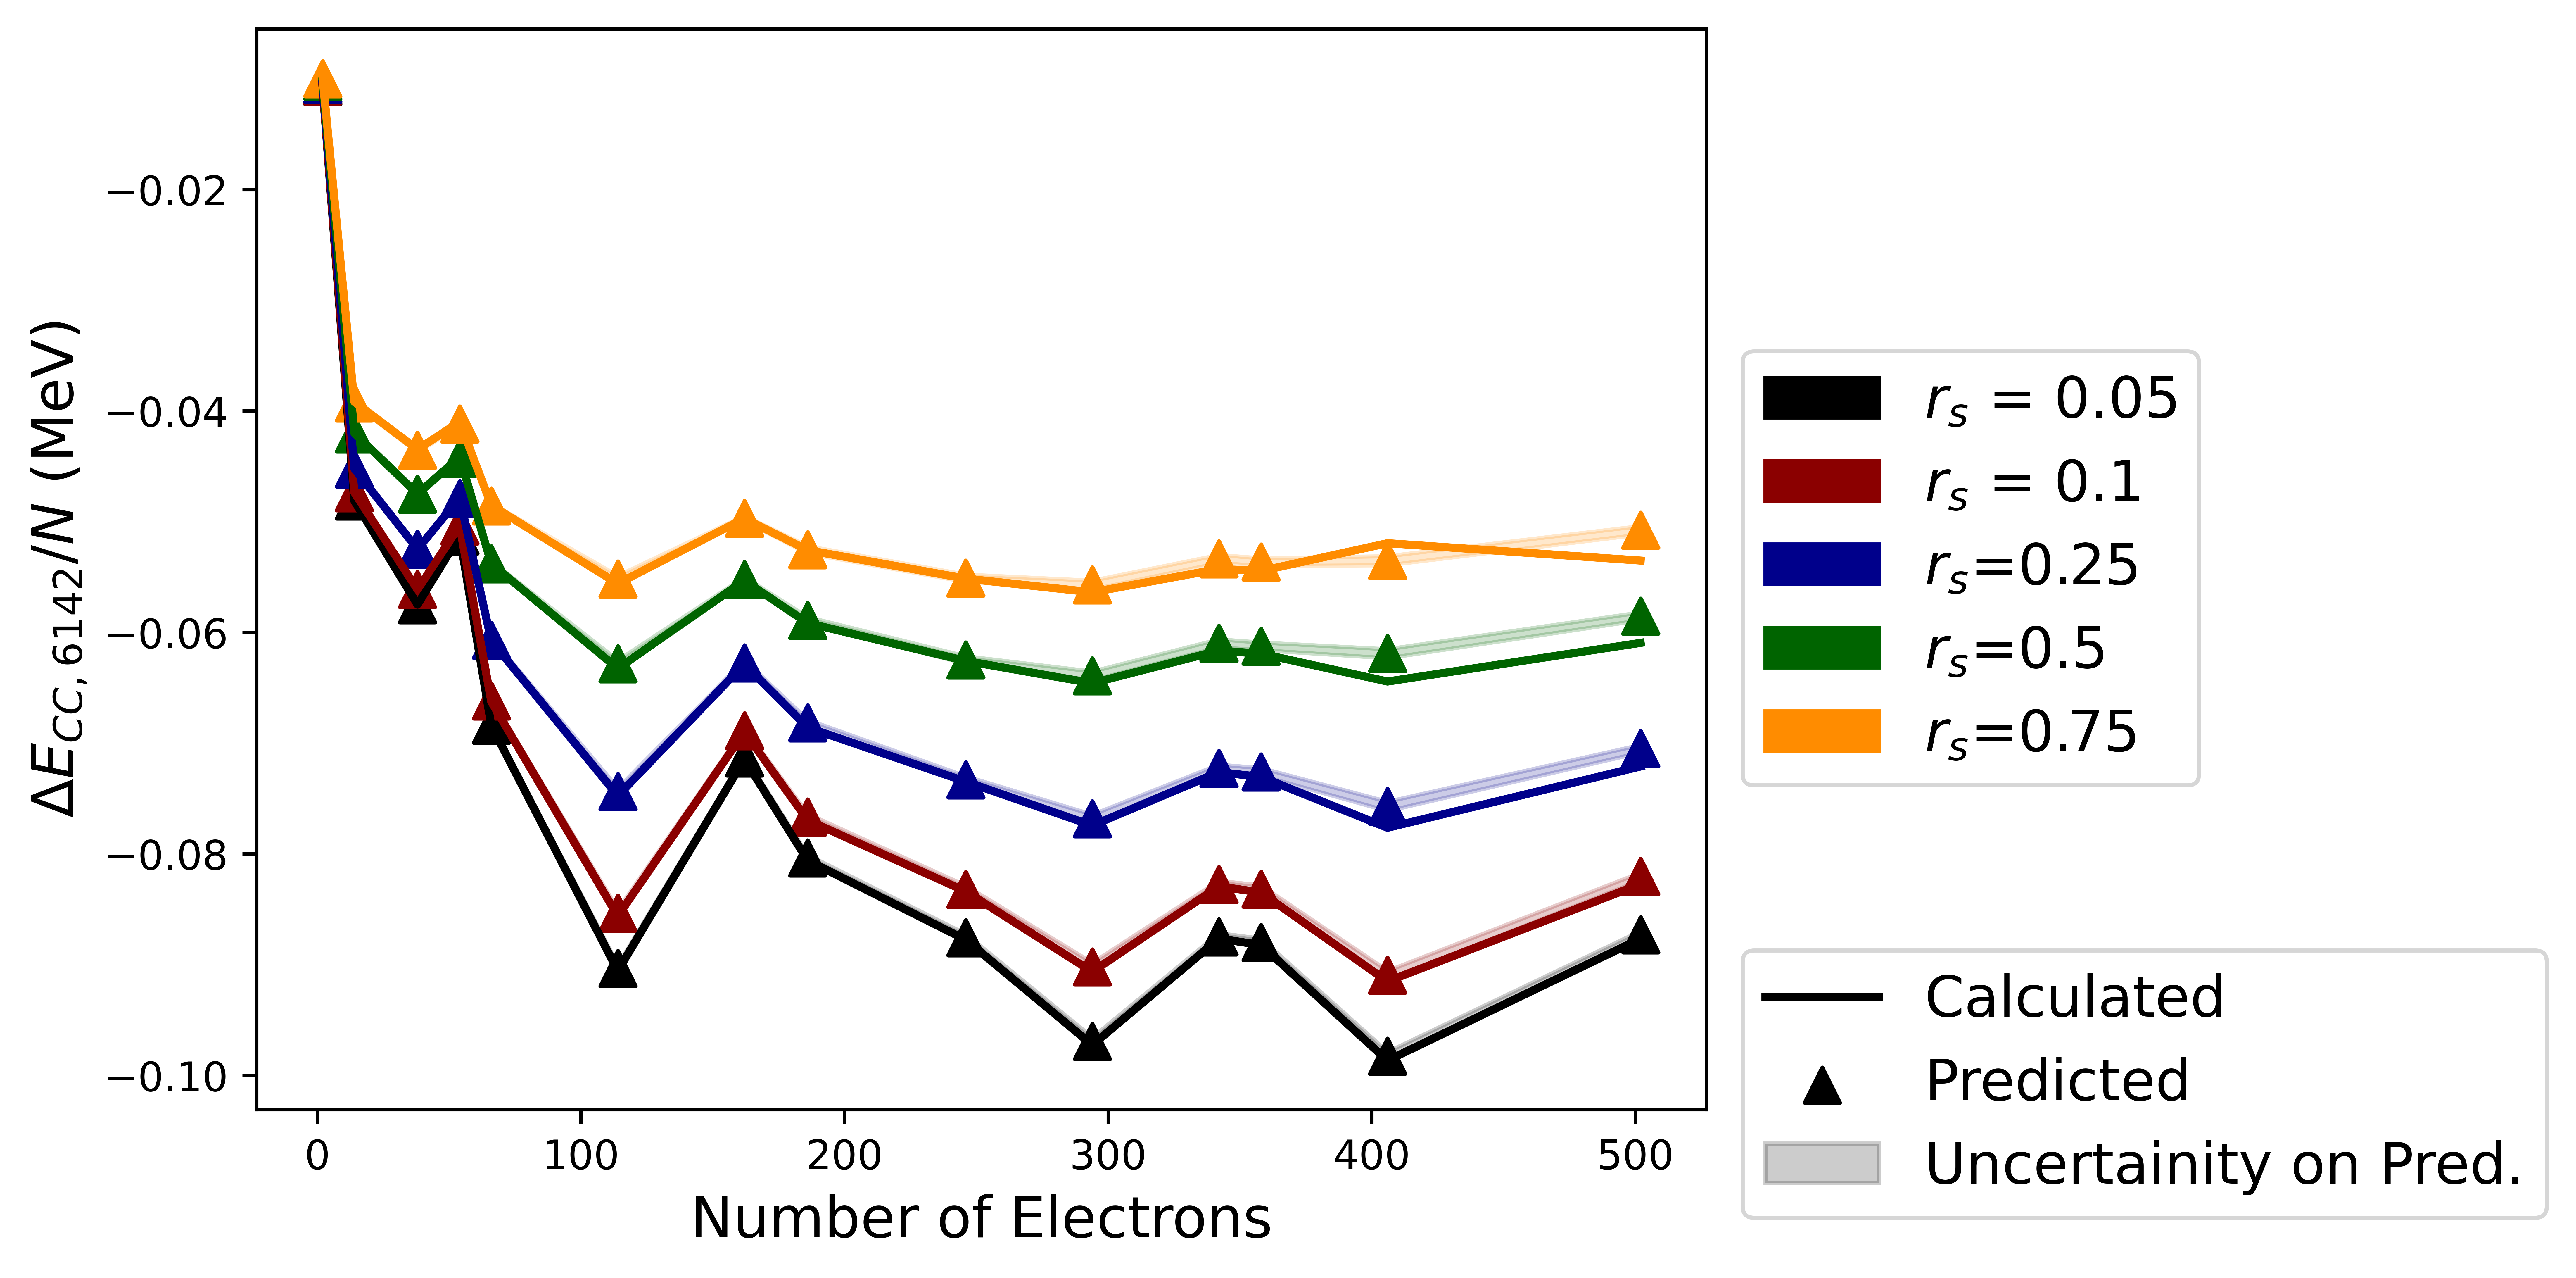
\includegraphics[scale=0.75]{Images/Chapter7/ElectronGas/BRR_EG_MSU_uncertainities-GP.png}
    \caption{The results of performing an SRE analysis with Gaussian processes to predict the converged correlation energies for the HEG at different values of N and $r_s$.  The correlation energies calculated at M = 6,142 are plotted with a solid line and are taken to be the true results, the SRE predictions are plotted with triangular markers, and the shaded region represents the uncertainty on the SRE predictions.}
    \label{fig:gp_16_points}
\end{figure}


As a final analysis with the SRE method on the HEG, we will again use GP as the machine learning algorithm but will reduce the number of training points from 16 to only 10. Here we will use data collected from 5 to 14 open shells, thus removing the six training points with the highest number of single-particle states (and thus the highest computational costs). Here we have also reduced the SRE sequence length to 1 as there are a few training points.

The results of performing this analysis are shown in Fig. \ref{fig:gp_10_points}, using the same plotting scheme as \ref{fig:gp_16_points}. The lower number of training points does lead to a higher average percent error of 1.16$\%$, but this is still a relatively low error, and it does appear, based on the results graph, that most of that error is concentrated in the last two points of the $r_s$ = 0.75 data set.

Next, we must point out the time savings we have gained by reducing the number of training points. When using 16 training points, the time savings is 88.99 node hours, which is not an insignificant amount of time saved. However, with only ten training points, and since the six training points we have removed have the most significant computational time, with this analysis, the amount of computational time saved is 224.43 node hours. That is equivalent to over a week in computational time saved for an error of only 1.16$\%$!

Finally, we justify using the Gaussian processes as the machine learning algorithm over Bayesian ridge regression when there is a small amount of training data. For example, suppose we were to perform this same analysis with Bayesian ridge regression, using ten training points and a sequence length of 1. In that case, the average percent error across all the correlation energies is 6.05$\%$, much higher than the 1.16$\%$ we see with GP. Thus, the GP algorithm works better with smaller data sets and will be the primary algorithm we will use in the next chapter to analyze the infinite nuclear matter, as no training set in that chapter will contain more than 10 points.

\begin{figure}
    \centering
    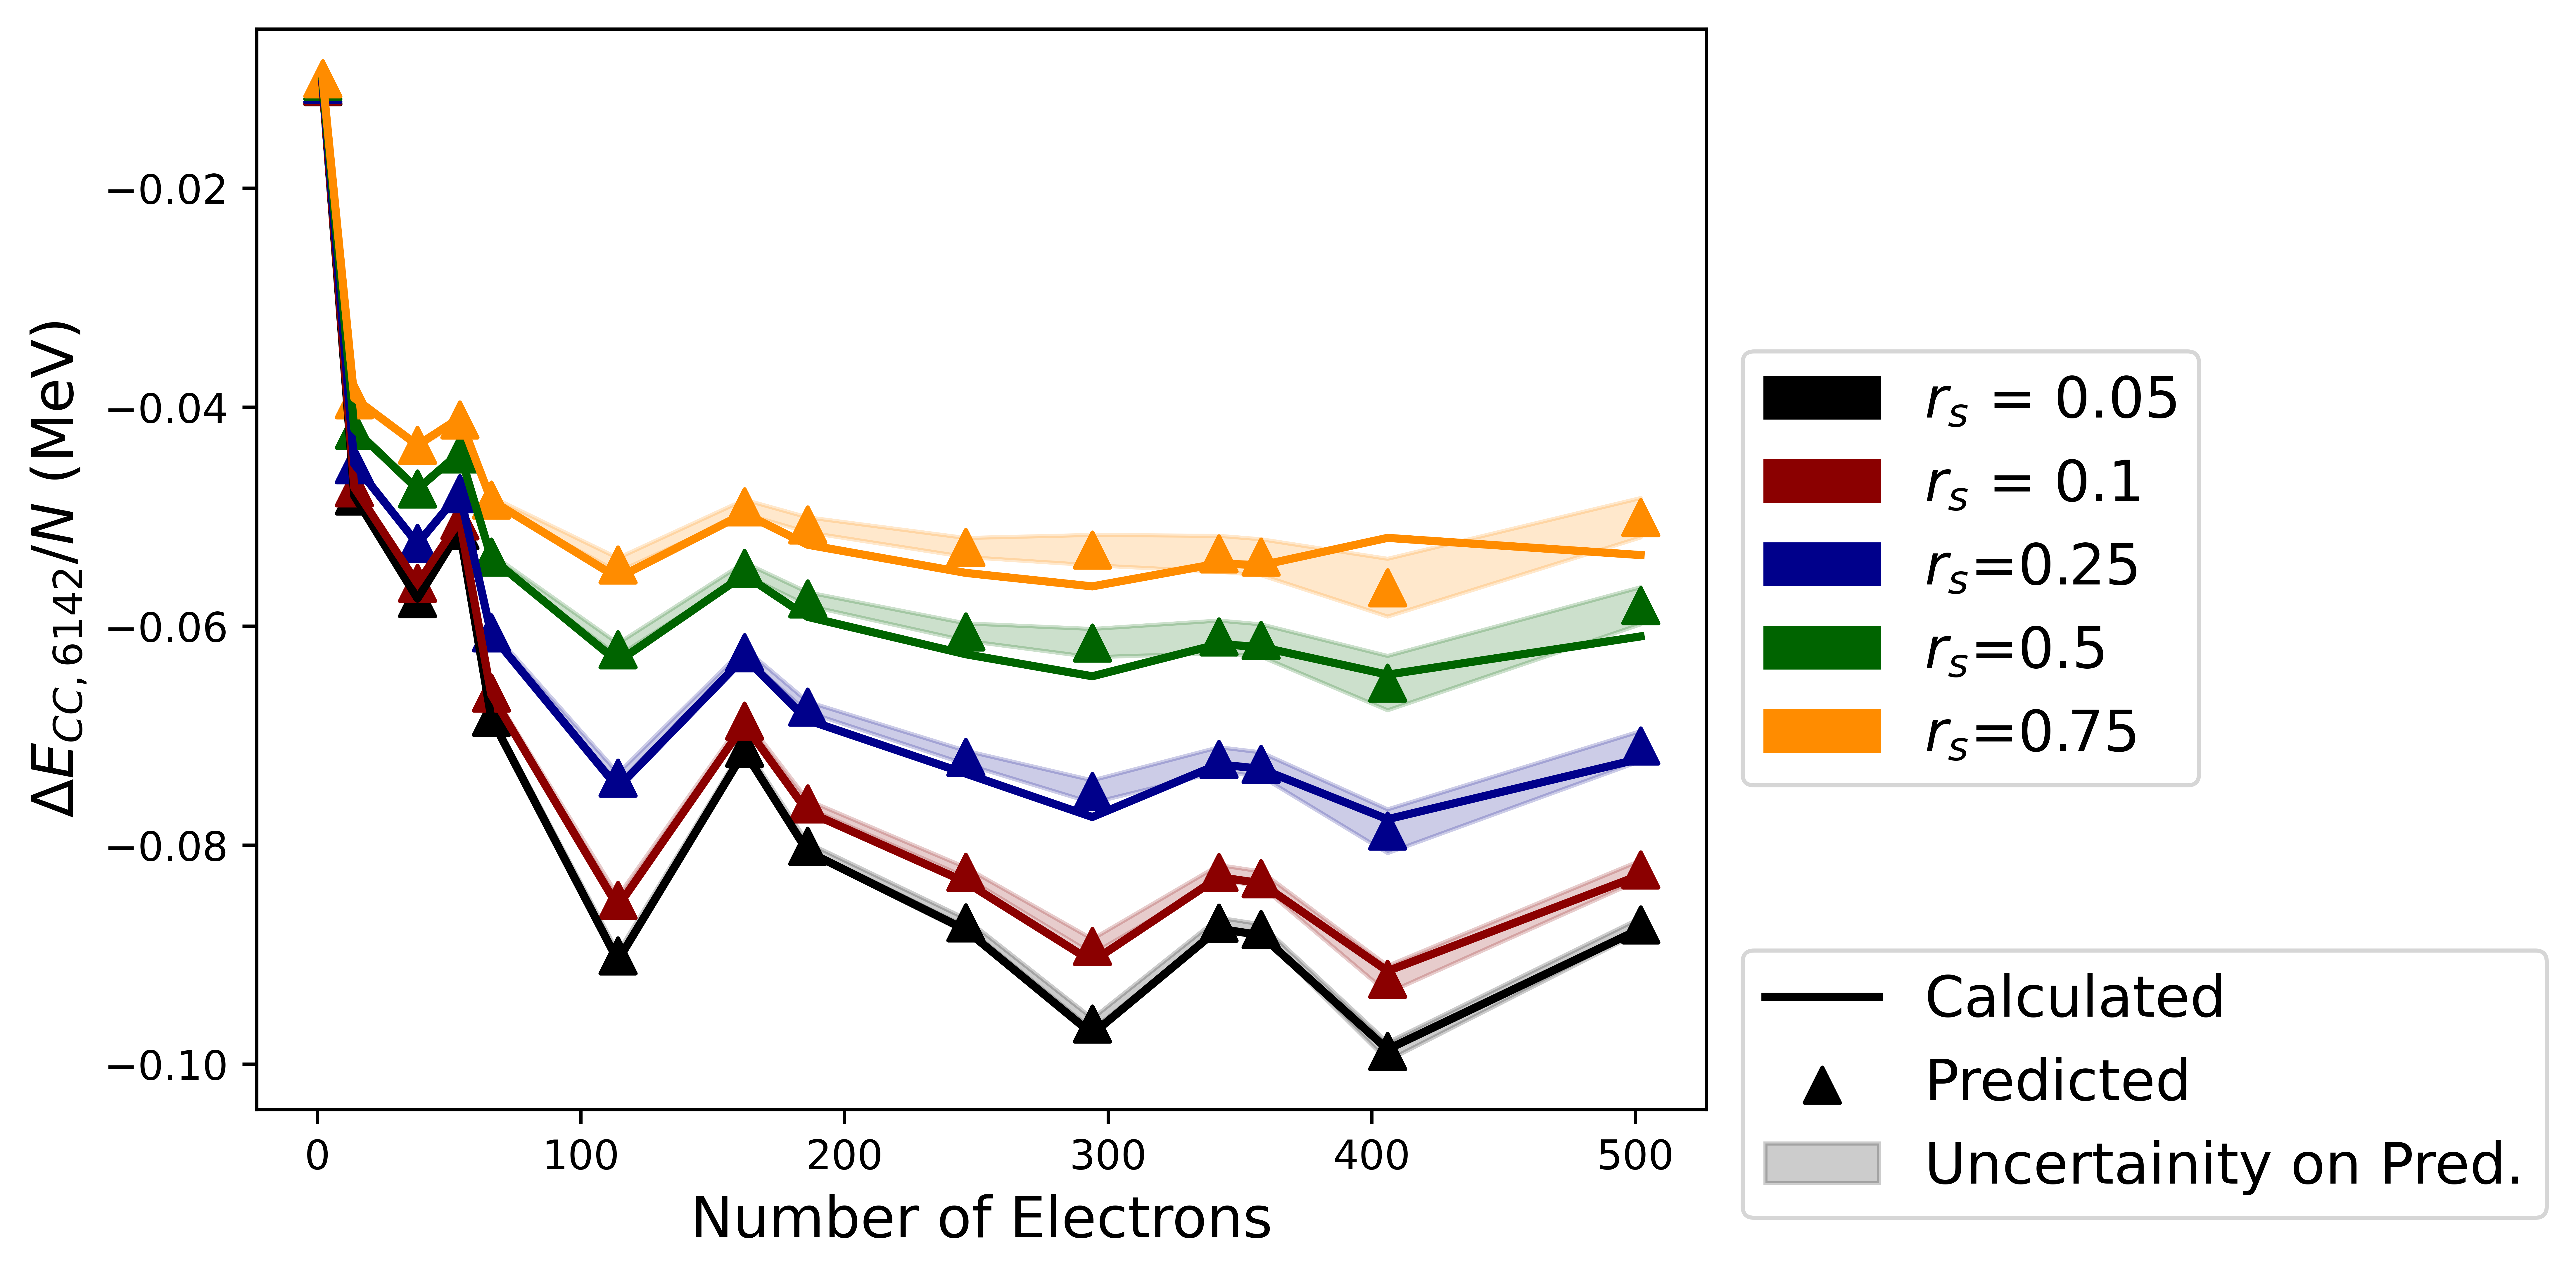
\includegraphics[scale=0.75]{Images/Chapter7/ElectronGas/BRR_EG_MSU_uncertainities_GP_2.png}
    \caption{The results of performing an SRE analysis with Gaussian processes to predict the converged correlation energies for the HEG at different values of N and $r_s$ and only ten training points.  The correlation energies calculated at M = 6,142 are plotted with a solid line and are taken to be the true results, the SRE predictions are plotted with triangular markers, and the shaded region represents the uncertainty on the SRE predictions.}
    \label{fig:gp_10_points}
\end{figure}